% Source : http://tex.stackexchange.com/questions/3892/how-do-you-draw-the-snake-arrow-for-the-connecting-homomorphism-in-the-snake-l

\documentclass{article}
\usepackage{tikz}
\usetikzlibrary{matrix,arrows}

\begin{document}

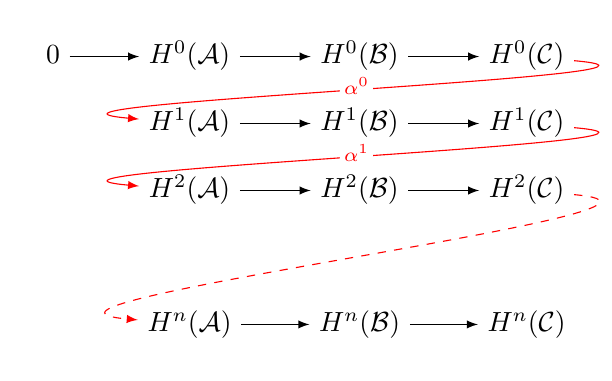
\begin{tikzpicture}[descr/.style={fill=white,inner sep=1.5pt}]
        \matrix (m) [
            matrix of math nodes,
            row sep=1em,
            column sep=2.5em,
            text height=1.5ex, text depth=0.25ex
        ]
        { 0 & H^0(\mathcal A) & H^0(\mathcal B) & H^0(\mathcal C) \\
            & H^1(\mathcal A) & H^1(\mathcal B) & H^1(\mathcal C) \\
            & H^2(\mathcal A) & H^2(\mathcal B) & H^2(\mathcal C) \\
            & \mbox{}         &                 & \mbox{}         \\
            & H^n(\mathcal A) & H^n(\mathcal B) & H^n(\mathcal C) \\
        };

        \path[overlay,->, font=\scriptsize,>=latex]
        (m-1-1) edge (m-1-2)
        (m-1-2) edge (m-1-3)
        (m-1-3) edge (m-1-4)
        (m-1-4) edge[out=355,in=175,red] node[descr,yshift=0.3ex] {$\alpha^0$} (m-2-2)
        (m-2-2) edge (m-2-3)
        (m-2-3) edge (m-2-4)
        (m-2-4) edge[out=355,in=175,red] node[descr,yshift=0.3ex] {$\alpha^1$} (m-3-2)
        (m-3-2) edge (m-3-3)
        (m-3-3) edge (m-3-4)
        (m-3-4) edge[out=355,in=175,dashed,red] (m-5-2)
        (m-5-2) edge (m-5-3)
        (m-5-3) edge (m-5-4);
\end{tikzpicture}

\end{document}
